\section{Resultados: base, mejora y sensibilidad}
\label{sec:resultados}

\begin{alcance}
Todo lo que sigue son resultados de \textbf{simulación} (\texttt{synthetic\_simulation}) con
parámetros calibrados con NHAMCS 2022 y un servicio supuesto. Describen una mejora
\emph{simulada}; no se observó ninguna mejora en un hospital.
\end{alcance}

\subsection{Condiciones y variabilidad}
La tabla~\ref{tab:condiciones} muestra la espera media de las seis condiciones con su
dispersión entre réplicas. La variación entre días simulados es grande: la desviación
estándar de la espera media nominal es \StdBaseNom{} min (base) y \StdCandNom{} min
(candidata), y los intervalos marginales del 95\,\% de la media
([\MargBaseLow, \MargBaseHigh] y [\MargCandLow, \MargCandHigh] min) se solapan. Por eso el
efecto del horario se estima con diferencias pareadas, que eliminan parte de la variación
compartida.

\begin{table}[ht]
\centering\small
\caption{Espera media por condición ($n=\NReps$ réplicas cada una). El drenaje es el tiempo
posterior al cierre de la ventana hasta que toda la cohorte medida inicia atención; no entra
en las métricas de cola ni de utilización.}
\label{tab:condiciones}
\fittable{generated/tab_conditions.tex}
\end{table}

\begin{figure}[ht]
\centering
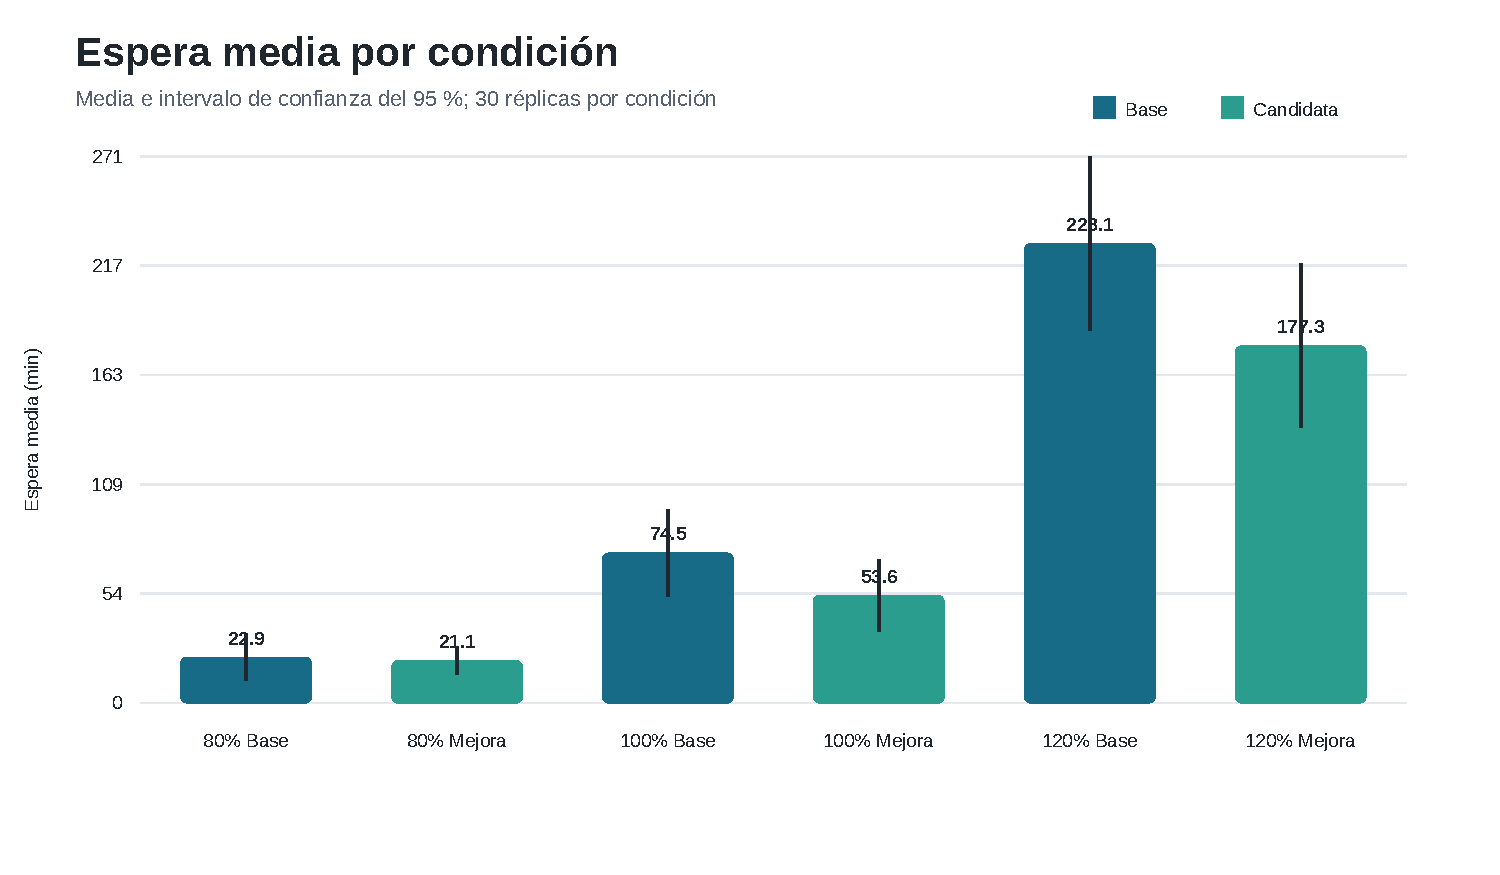
\includegraphics[width=0.92\linewidth]{figures/mean_wait_by_condition.pdf}
\caption{Espera media por condición, con intervalo de confianza del 95\,\% (30 réplicas por
condición). Figura generada en \texttt{evidence/final/figures/}.}
\label{fig:condiciones}
\end{figure}

\subsection{Efecto del horario sobre la espera media}
\begin{table}[ht]
\centering\small
\caption{Diferencia pareada de la espera media (base $-$ candidata). Valores positivos
indican menos espera con la candidata. El intervalo es normal del 95\,\% para la media de las
\NReps{} diferencias pareadas.}
\label{tab:pareada}
\fittable{generated/tab_paired_mean_wait.tex}
\end{table}

\begin{figure}[ht]
\centering
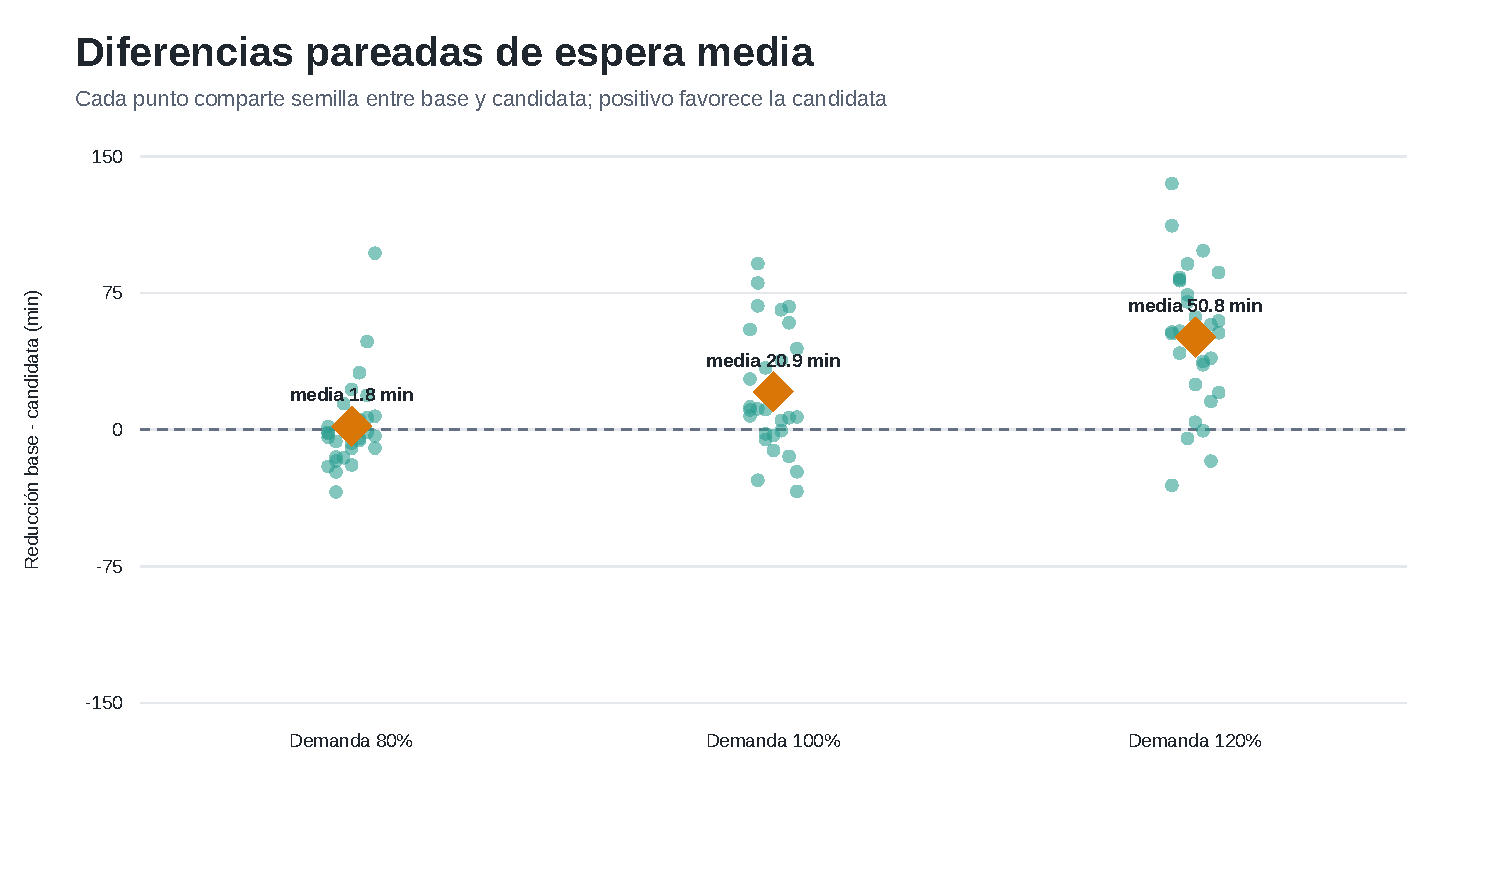
\includegraphics[width=0.92\linewidth]{figures/paired_wait_improvement.pdf}
\caption{Distribución de la mejora pareada de la espera media por nivel de demanda
(figura generada en \texttt{evidence/final/figures/}).}
\label{fig:pareada}
\end{figure}

La reducción es de \RedNom{} min (\RedPctNom\,\%) con demanda nominal y de \RedHigh{} min
(\RedPctHigh\,\%) con demanda alta; en ambos casos el intervalo pareado excluye el cero y la
candidata favorece a \PairsPosNom{} y a \PairsPosHigh{} de las \NReps{} parejas, respectivamente.
Con demanda baja la reducción media es de \RedLow{} min, el intervalo
([\RedCILowLow, \RedCIHighLow]) incluye el cero y solo \PairsPosLow{} de \NReps{} parejas
favorecen a la candidata: \textbf{no se afirma una mejora consistente} en esa condición.
El mayor efecto absoluto aparece cuando el sistema está más exigido.

\subsection{Otras métricas}
\begin{table}[ht]
\centering\small
\caption{Métricas bajo demanda nominal. El cambio es candidata $-$ base; el intervalo de la
última columna corresponde a la reducción pareada (base $-$ candidata).}
\label{tab:nominal}
\fittable{generated/tab_nominal.tex}
\end{table}

\begin{table}[ht]
\centering\small
\caption{Sensibilidad a la demanda del percentil 90, de la proporción con espera mayor a 60
minutos y de la cola media. Reducción = base $-$ candidata (intervalo pareado del 95\,\%).}
\label{tab:sensibilidad}
\fittable{generated/tab_secondary_by_demand.tex}
\end{table}

Con demanda nominal la candidata reduce también la mediana (\NomBaseMedian{} a
\NomCandMedian{} min), el percentil 90 (\NomBasePninety{} a \NomCandPninety{} min), la
proporción con espera mayor a 60 minutos (\NomBaseShare{} a \NomCandShare{}) y la cola media
(\NomBaseQueue{} a \NomCandQueue{} pacientes). El resultado no se obtiene con más recursos: ambos
horarios usan 23 unidades. La utilización efectiva de la candidata es ligeramente menor, lo
que refleja una mejor coincidencia temporal entre demanda y capacidad, no capacidad adicional.

\subsection{Congestión terminal}
El drenaje medio tras el cierre de la ventana es de \DrainBaseNom{} min en la base y
\DrainCandNom{} min en la candidata bajo demanda nominal, y sube a \DrainBaseHigh{} y
\DrainCandHigh{} min con demanda alta. Las esperas se reportan completas (sin censura), pero
esos drenajes prolongados muestran saturación y limitan la extrapolación de la condición
de demanda alta.
